\documentclass[a4paper,fleqn,usenatbib]{mnras}

\usepackage{graphicx}	% Including figure files
\usepackage{amsmath}	% Advanced maths commands
\usepackage{amssymb}	% Extra maths symbols

\title[Human and machine classifications]{A transient search using combined human and machine classifications}

\author[D. Wright, C. Lintott et al.]{
Daryll Wright,$^{1}$\thanks{E-mail: daryll@zooniverse.org}
Chris Lintott,$^{2}$

$^{1}$Department of Physics, University of Oxford, Denys Wilkinson Building, Keble Road, Oxford, OX1 3RH
}

\date{Accepted XXX. Received YYY; in original form ZZZ}

\pubyear{2016}

\begin{document}
\label{firstpage}
\pagerange{\pageref{firstpage}--\pageref{lastpage}}
\maketitle

% Abstract of the paper
\begin{abstract}
Large modern surveys require efficient review of data in order to find transient sources such as supernovae, and to distinguish such sources from artefacts, noise and so on. Much effort has been put into the development of automatic algorithms, but surveys still rely on human review of targets. This paper presents an integrated system for the identification of supernovae in data from PanSTARRS, combining classifications from a citizen science project including volunteers with those from a convolutional neural network. This work represents the first time such a system has been deployed on real astronomical data, and we show that the combination of the two methods outperforms either one used individually. This result has important implications for the future development of transit searches, especially in the era of LSST and other large-throughput surveys. 
\end{abstract}

\begin{keywords}
keyword1 -- keyword2 -- keyword3
\end{keywords}

%%%%%%%%%%%%%%%%%%%%%%%%%%%%%%%%%%%%%%%%%%%%%%%%%%

%%%%%%%%%%%%%%%%% BODY OF PAPER %%%%%%%%%%%%%%%%%%

\section{Introduction}


\begin{figure}
   %\vspace{200pt}
   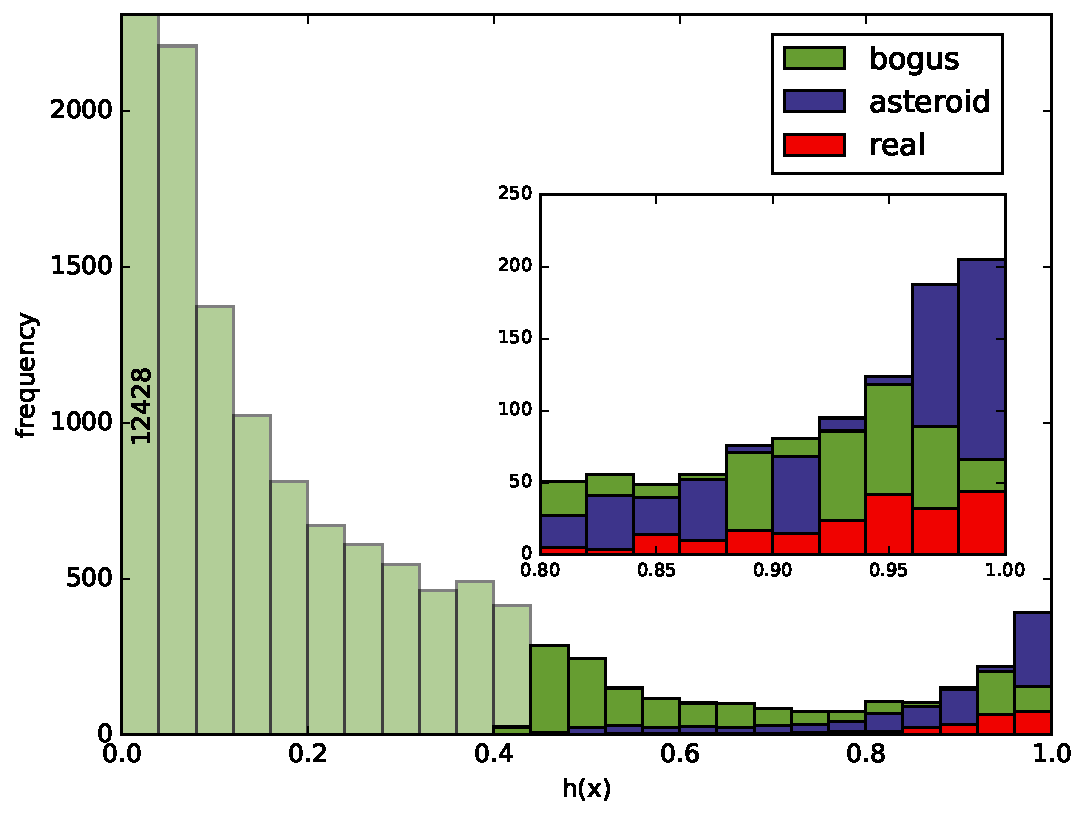
\includegraphics[width=84mm]{figs/machine_hist.pdf}
   \caption{The distribution of $P(real)$ from the current 3$\pi$ machine classifier 
            for detected objects between MJD 57570 and MJD 57586.  The light green shows the distribution of 
            objects with $P(real) < 0.436$ which are automatically rejected.  The remaining 
            objects promoted for human screening even at high values of $P(real)$ contains
            many false positives.} 
   \label{fig:machine_dist} 
\end{figure}


\begin{figure}
   %\vspace{200pt}
   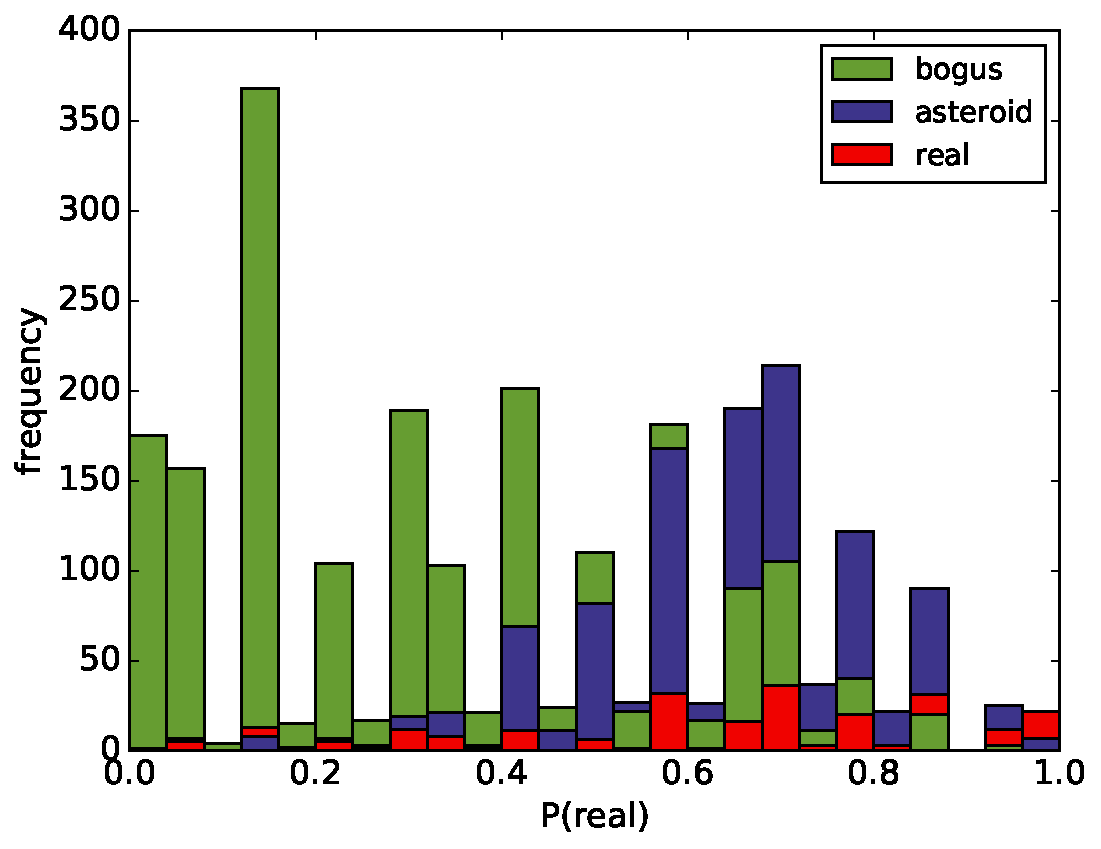
\includegraphics[width=84mm]{figs/human_hist.pdf}
   \caption{The distribution of $P(real)$ from Supernova Hunters for objects detected between 
            MJD 57570 and MJD 57586.  Compared with the machine $P(real)$ in ~\ref{fig:machine_dist}
            the objects at the extremes are pure.  There are very few real detections with 
            $P(real) < 0.04$ and few bogus detections above 0.92.} 
   \label{fig:human_dist} 
\end{figure}

\begin{figure}
   %\vspace{200pt}
   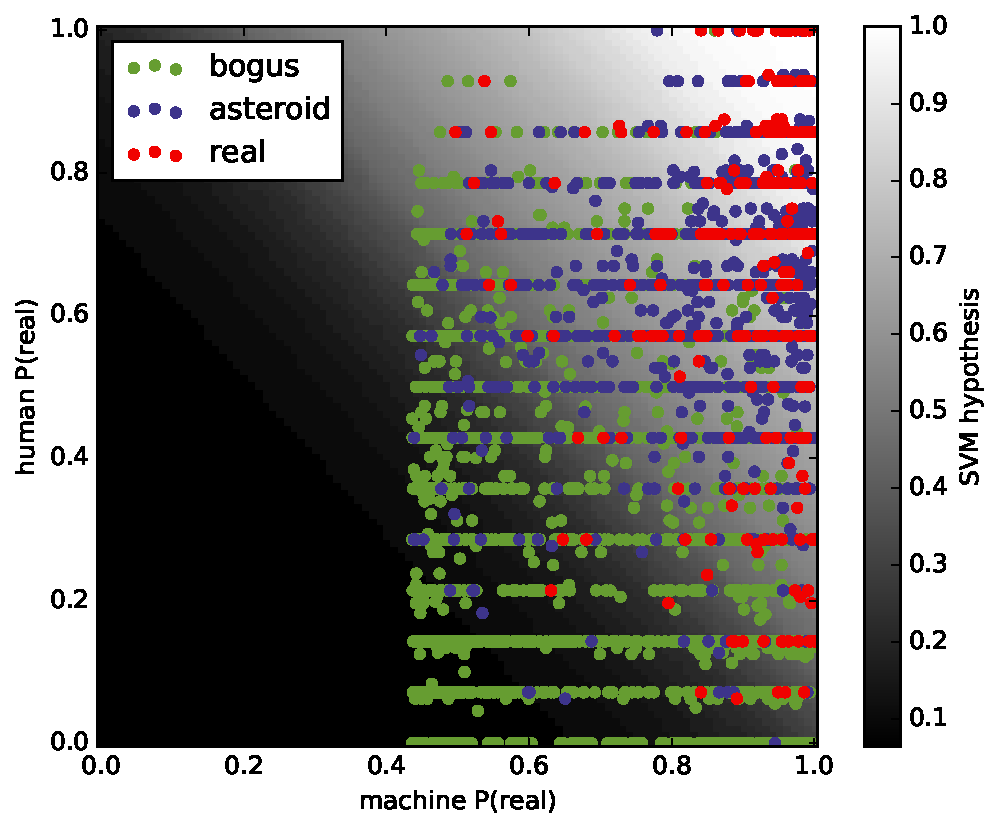
\includegraphics[width=84mm]{figs/human_v_machine_train.pdf}
   \caption{The $P(real)$ from Supernova Hunters against the machine $P(real)$ for detected 
            objects between MJD 57570 and MJD 57586.  Objects with machine $P(real) < 0.436$ are
            not uploaded to Supernova Hunters.  The background colour map shows 
            the $P(real)$ to that point in feature space by a linear SVM trained on the 
            examples shown.}
   \label{fig:combo_train} 
\end{figure}

\begin{figure}
   %\vspace{200pt}
   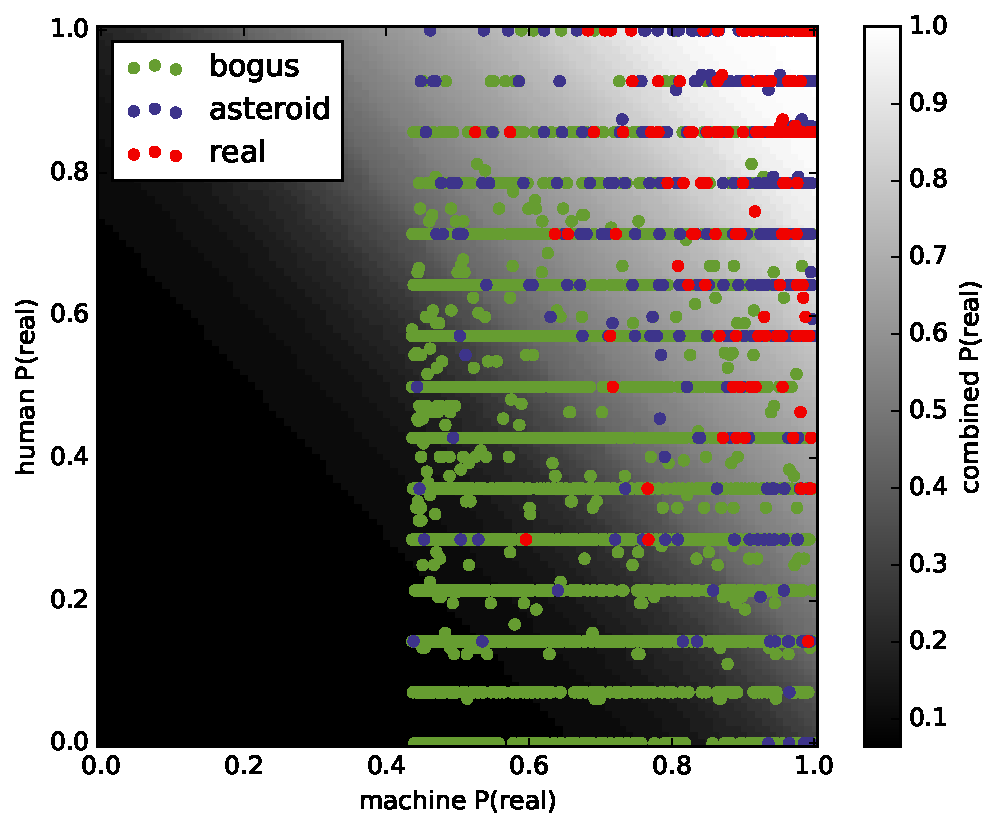
\includegraphics[width=84mm]{figs/human_v_machine_test.pdf}
   \caption{The same as ~\ref{fig:combo_train} but on a test sample of 4058 objects detected between
            MJD 57587 and MJD 57607 and held out during training of the linear SVM.} 
   \label{fig:combo_test} 
\end{figure}

\begin{figure}
   %\vspace{200pt}
   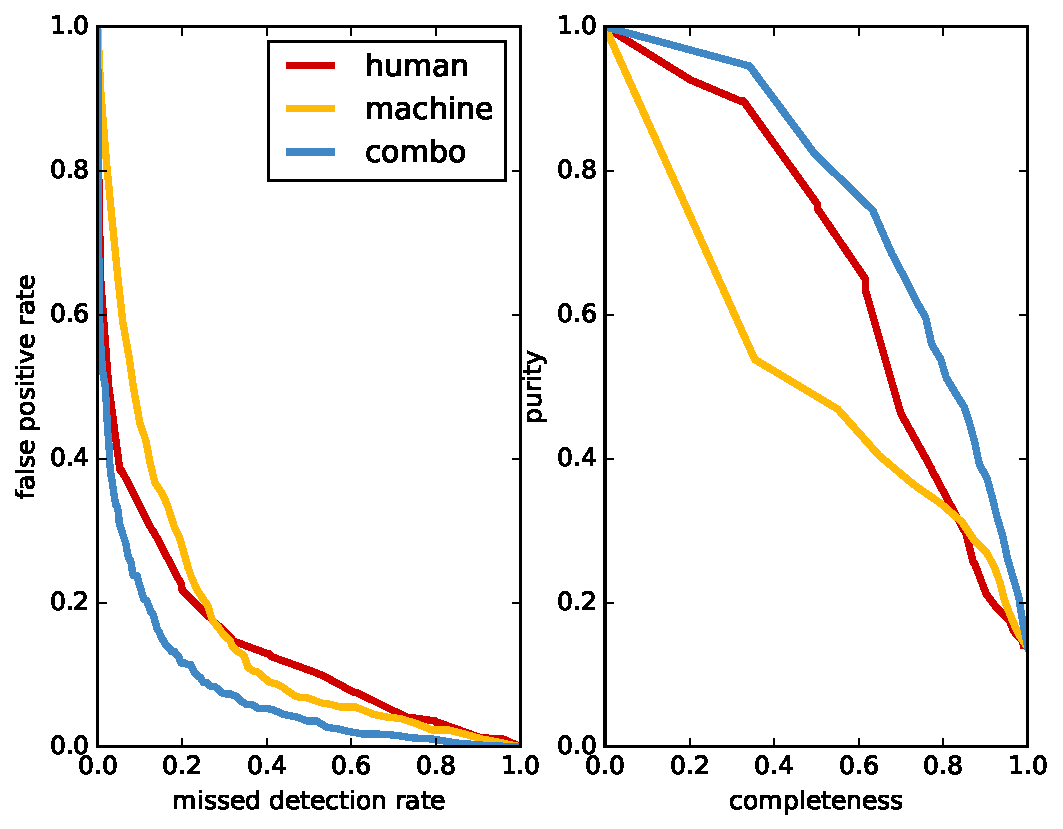
\includegraphics[width=84mm]{figs/roc.pdf}
   \caption{left: ROC curve showing performance measured on the test data in ~\ref{fig:combo_test} for human (red), machine (yellow) and
            the linear SVM combination of human and machine classifications (blue).  right: The equivalent Purity-Completeness curve.  Both
            plots show that the combination is always as good as or outperforms humans or the machine individually.} 
   \label{fig:roc} 
\end{figure}

\bsp	% typesetting comment
\label{lastpage}
\end{document}